\section{Uživatelská dokumentace}

Tato kapitola obsahuje uživatelskou dokumentaci aplikace.

Aplikace umožňuje vytváření a správu výukových kurzů, kterýkoliv uživatel si může vytvořit vlastní kurz.
Kurz může představovat vysokoškolskou přednášku, cvičení, předmět na střední škole nebo také jazykový, příp. jiný zájmový kurz.

V kurzu jsou dva typy uživatelů:
\begin{itemize}
	\item Studenti
	\item Administrátoři (správci)
\end{itemize}

Role se vztahuje pouze k danému kurzu, uživatel tedy může být v jednom kurzu administrátor, v jiném naopak pouze student. 
Administrátoři mohou měnit obsah kurzu (přidávat, odebírat materiály, apod.) a vytvářet nové testy. 
Testy dělíme na dva typy:

\begin{itemize}
	\item Hodnocené testy
	\item Nehodnocené testy (kvízy)
\end{itemize}

Rozdíl je v tom, že kvízy se nepočítají do celkového hodnocení studenta.

Studenti daného kurzu pak mohou testy vyplňovat a zobrazit si své známky i opravená řešení.
Systém vyhodnocuje řešení testů automaticky, nicméně správci kurzu mohou následně body upravit ručně. 

Testy se skládají z jednotlivých otázek, ty dělíme na tři typy podle druhu odpovědí.
\begin{itemize}
	\item textová odpověď
	\item výběr z nabídky odpovědí -- právě jedna z nabízených odpovědí je správná
	\item vícenásobný výběr z nabídky odpovědí -- více nabízených odpovědí může být správných
\end{itemize}

V prvních dvou typech otázek probíhá vyhodnocení jednoduše, pokud se odeslaná a správná odpověď shodují, systém udělí za tuto otázku plný počet bodů, v opačném případě neudělí žádné body.
V případě vícenásobného výběru z odpovědí systém nejprve spočítá počet správných voleb (tzn. vybraných odpovědí, které jsou správné a nevybraných odpovědí, které jsou chybné).
Dále spočítá procentuální poměr správných voleb a udělí procentuálně daný počet bodů za tuto otázku.
Pro ilustraci uvedeme příklad s otázkou, která je hodnocena šesti body, a obsahuje tři možné odpovědi, z nichž dvě jsou správné. Student zaškrtne pouze jednu správnou odpověď (ostatní možnosti nevybere), za otázku tedy dostane $\frac{2}{3} * 6 = 4$ body.

Dále mohou administrátoři přidělovat studentům i známky, které se nevážou k žádnému testu, což můžeme využít například k reprezentaci známek za aktivitu v hodině.
Aplikace používá k hodnocení procenta, jednotlivé testy a známky mohou mít různou váhu. 

Na obrázku \ref{fig:login} vidíme uživatelské rozhraní aplikace.

\vspace{\baselineskip}

Následující podkapitoly obsahují jednotlivé uživatelské scénáře rozepsané v bodech a doplněné snímky obrazovky.

\subsection{Registrace nového uživatele}

\begin{itemize}
	\item Pro registraci nového uživatele nejprve klikneme na tlačítko Register v horním menu.
	\item Uživatelé v aplikaci jsou identifikováni pomocí e-mailu. Do registračního formuláře zadáme tedy e-mail a heslo nového uživatele, a stiskneme tlačítko Register.
	\item Zobrazí se stránka s potvrzením registrace. Vzhledem k našim potřebám aktuálně neprovádíme ověření e-mailu. Pokud bychom chtěli tuto funkcionalitu přidat, můžeme postupovat například podle návodu v dokumentaci. \cite{AspNetCoreDocs} Klikneme na odkaz s textem 'Click here to confirm your account', a tím je registrace dokončena. Pomocí odkazu pak můžeme přejít na stránku s přihlášením.
\end{itemize}

\subsection{Přihlášení uživatele}

\begin{itemize}
	\item Pro přihlášení uživatele nejprve stiskneme tlačítko Login v horním menu.
	\item Zobrazí se přihlašovací formulář, do kterého vyplníme e-mail a heslo, jak můžeme vidět na obrázku \ref{fig:login}
	\item Po odeslání formuláře nás aplikace přihlásí a přesměruje na stránku se seznamem kurzů.
	\item Pokud se následně chceme odhlásit, vybereme v menu volbu Logout.
\end{itemize}

\subsection{Zobrazení stránky se seznamem kurzů}

\begin{itemize}
	\item Po kliknutí na odkaz Courses v menu se zobrazí stránka, na které se nachází seznam kurzů. (viz. obrázek \ref{fig:courses-list})
	\item Na této stránce se nachází několik sekcí. Sekce Member courses obsahuje všechny kurzy, jejichž jsme členy. Po kliknutí na odkaz s názvem kurzu se dostaneme na stránku s detaily kurzu.
	\item Sekce Managed courses obsahuje všechny kurzy, které spravujeme (tzn. jsme administrátoři). Kliknutím na odkaz s názvem kurzu se opět dostaneme na stránku s detaily kurzu. Každý z těchto kurzů můžeme také smazat -- kliknutím na tlačíko "Delete" vedle názvu kurzu.
	\item Dále se na této stránce nachází sekce, které slouží k přidání nového kurzu a zápisu do kurzu (více viz. dále). Úplně dole je pak sekce, ve které můžeme vidět náš uživatelský identifikátor.
\end{itemize}

\subsection{Vytvoření nového kurzu}

\begin{itemize}
	\item Na stránce se seznamem kurzů je sekce s názvem Add new course, která obsahuje formulář pro přidání nového kurzu.
	\item Do políčka Name vyplníme jméno kurzu a klikneme na tlačítko Add.
	\item Vytvoří se nový kurz, který má právě jednoho administrátora -- nás.
\end{itemize}

\subsection{Zápis do kurzu}

\begin{itemize}
	\item Nejprve přejdeme na stránku se seznamem kurzů a vybereme sekci Enroll to a course.
	\item K přihlášení do kurzu je nejprve třeba znát jeho identifikátor, ten nám může například zaslat nějaký z administrátorů. Po získání identifikátoru jej vložíme do políčka s názvem 'Course ID' a formulář odešleme kliknutím na tlačítko Enroll.
	\item Tímto vytvoříme žádost o přihlášení do daného kurzu. Členem kurzu se staneme až poté, co nám žádost schválí některý z administrátorů.
\end{itemize}

\subsection{Zobrazení detailu kurzu}

\begin{itemize}
	\item Po kliknutí na kurz v seznamu kurzů se dostaneme na stránku s detaily.
	\item Úplně nahoře vidíme sekci s názvem kurzu (viz. obrázek \ref{fig:course-detail}) , ve které se zároveň nachází identifikátor tohoto kurzu, který se používá při zápisu do kurzu. Členové kurzu zde také vidí tlačítko s textem 'My Grades', pomocí kterého se dostanou na stránku s hodnocením studenta.
	\item Pod touto sekcí se nachází seznam testů, rozdělený do tří kategorií:
		\begin{itemize}
			\item Not Published -- tyto testy zatím nebyly publikované, mohou si je zobrazit pouze administrátoři.
			\item Active -- tyto testy jsou aktivní, aktuálně je lze odevzdávat.
			\item After deadline -- testy, které již není možné odevzdat.
		\end{itemize}
		Pokud některá z kategorií neobsahuje žádný test, tak se na stránce vůbec nezobrazuje. Studenti kurzu vidí pouze kategorii 'Active', zatímco administrátorům se zobrazují všechny tři výše uvedené kategorie.
		
		U každého testu je uvedena informace, jestli je hodnocený (GRADED, příp. NOT GRADED) a případně i deadline.
		Po kliknutí na název testu se student dostane buď na stránku s odevzdáním, anebo na stránku s vyhodnoceným řešením, pokud již test odevzdal. Administrátory kurzu aplikace přesměruje na stránku s detaily testu.
		
	\item Na stránce je dále sekce se sdílenými soubory, které si můžeme stáhnout. Správci kurzu zde vidí i formulář pro nahraní nového souboru.
	\item Dále se zde nachází komponenty se seznamy členů a administrátorů daného kurzu, které se zobrazují pouze administrátorům (více viz. dále).
	\item Na stránce dále můžeme vidět fórum s příspěvky. U každého příspěvku je uvedený text a jeho autor. Správci kurzu zde vidí také tlačítko pro smazání příspěvku.
	\item Pod fórem se nachází formulář, pomocí kterého lze přidávat nové příspěvky.
	\item Úplně dole je pak tlačítko, které slouží k opuštění kurzu. Tato akce je nevratná, pokud tedy kurz opustíme, nemůžeme původní účet v aplikaci nijak obnovit. Můžeme ovšem zažádat o nové zapsání do kurzu.
\end{itemize}

\subsection{Zobrazení detailu studenta}

\begin{itemize}
	\item Na stránku s detaily studenta se můžeme dostat ze stránky s detaily kurzu. Studenti si stránku mohou zobrazit pomocí tlačítka 'My Grades', administrátoři se sem dostanou pomocí kliknutí na detail studenta v sekci s členy kurzu.
	\item Na obrázku \ref{fig:student-detail}, vidíme, že na této stránce se nachází komponenty s hodnocením daného studenta. 
	\item Nachází se zde tabulka s odevzdanými testy, po kliknutí na název testu se dostaneme na stránku s vyhodnoceným řešením. U každého testu pak vidíme získané skóre, váhu testu (tedy dopad na celkovou známku), datum a čas odevzdání. Poslední sloupec nám říká, jestli bylo odevzdané řešení již revidované
	\item Pod seznamem odevzdaných testů se nachází komponenta s dalšími známkami. Tyto známky nepatří k žádnému testu. 
	\item Na stránce se dále nachází sekce s celkovým skóre studenta, ve které můžeme vidět vážený průměr všech jeho známek.
	\item Pod touto sekcí se nachází formulář pro přidávání známek, který se zobrazuje pouze administrátorům.
	\item Ve spodní části stránky je komponenta s odevzdanými kvízy (tzn. nehodnocenými testy). Po kliknutí na název kvízu nás aplikace přesměruje na detail odevzdaného řešení.
\end{itemize}

\subsection{Odevzdání testu}

\begin{itemize}
	\item Nejprve přejdeme na stránku nějakého kurzu, jehož jsme členy.
	\item V seznamu testů vybereme ten, který chceme odevzdat.
	\item Pokud jsme tento test zatím neodevzdali, aplikace nás přesměruje na stránku s odevzdáním daného testu, jak můžeme vidět na obrázku \ref{fig:test-submit}. V případě, že jsme test již odevzdali, zobrazí se stránka s vyhodnoceným řešením.
	\item V horní části vidíme název testu, deadline -- čas, do kterého je třeba test odevzdat a několik dalších informací. Test následně vyplníme, u některých otázek máme na výběr z možností odpovědí.
	\item Stisknutím tlačítka Save answers dojde k uložení odpovědí. Můžeme tedy stránku opustit, příp. zavřít a při dalším načtení stránky se načtou i uložené odpovědi.
	\item Odevzdání testu provádíme pomocí tlačítka Submit. Tato akce je nevratná, po odevzdání testu jej není možné nijak upravovat ani znovu odevzdat.
	\item Po odevzdání testu jej systém vyhodnotí a aplikace nás přesměruje na stránku s vyhodnoceným řešením.
\end{itemize}

\subsection{Zobrazení vyhodnoceného testu}

\begin{itemize}
	\item Na obrázku \ref{fig:submission-review} vidíme příklad stránky s vyhodnoceným řešením testu.
	\item Ve vrchní části stránky je komponenta s informacemi o testu. Nachází se zde název testu, informace o tom, jestli je test hodnocený a přesný čas odeslání. Pokud byl test již revidován, nachází se zde i řetězec 'Reviewed'. 
	\item Na stránce se dále nachází seznam otázek. U každé otázky se zobrazuje text, udělené body, odeslaná a správná odpověď, a případně i komentář opravujícího.
	\item Pozadí otázky může mít různé barvy, podle toho, kolik bodů student z otázky získal.
		\begin{itemize}
			\item Zelená -- otázka je zodpovězena správně.
			\item Červená -- otázka je zodpovězena špatně, student z této otázky tedy nezískal žádné body.
			\item Oranžová -- otázka je zodpovězena částečně správně, student z této otázky tedy získal nějaké body, ale méně než plný počet.
		\end{itemize}
	\item Pod sekcí s otázkami se nachází komponenta, která slouží k revizi odeslaného řešení a je zobrazena pouze administrátorům.
	\item V dolní části stánky je sekce s hodnocením, ve které jsou uvedené získané body a skóre v procentech.
\end{itemize}

\subsection{Postranní menu s názvem kurzu}
 \begin{itemize}
 	\item Můžeme si všimnout, že na některých stránkách (například detail testu, detail studenta, jak můžeme vidět na obrázku \ref{fig:side-menu}) se zobrazuje postranní menu s názvem kurzu.
 	\item Pomocí odkazu v tomto menu se můžeme kdykoliv vrátit zpět na stránku příslušného kurzu.
 \end{itemize}


Následující akce mohou vykonávat pouze administrátoři příslušného kurzu.

\subsection{Administrace členů kurzu}

 \begin{itemize}
	\item Přejdeme na stránku daného kurzu.
	\item Pod sekcí se soubory se nachází komponenty, které obsahují seznamy studentů a administrátorů tohoto kurzu (viz. obrázek \ref{fig:students-admins-list}). 
	\item Pomocí tlačítka Details můžeme přejít na stránku s detaily tohoto studenta, naopak tlačítko Remove slouží k odstranění osoby z kurzu.
	\item Pod seznamem studentů se nachází tlačítko Enrollment Requests, které nám umožňuje zobrazit všechny žádostí o zapsání do tohoto kurzu.
	\item Komponenta s administrátory vypadá podobně, tlačítko Remove slouží k odebrání daného administrátora.
	\item Pod seznamem administrátorů se nachází formulář pro přidání nových administrátorů.
\end{itemize}

\subsection{Přidání nového administrátora do kurzu}

\begin{itemize}
	\item Přejdeme na stránku daného kurzu a najdeme sekci s administrátory.
	\item Nejprve potřebujeme zjistit identifikátor daného uživatele, ten může uživatel získat například na stránce se seznamem kurzů a poté nám jej zaslat.
	\item Vyplníme tento identifikátor do jediného políčka formuláře a potvrdíme stisknutím tlačítka Add.
	\item Pokud je požadavek úspěšně dokončen, přidá aplikace tohoto uživatele mezi administrátory kurzu.
\end{itemize}

\subsection{Sdílení souboru v kurzu}
\begin{itemize}
	\item Přejdeme na stránku daného kurzu a najdeme sekci se soubory.
	\item Ve formuláři pro přidání nového souboru klikneme na tlačítko s textem "Choose file".
	\item Vybereme soubor, který chceme sdílet a formulář potvrdíme.
	\item Soubor se následně zobrazí v seznamu sdílených souborů, který je dostupný všem členům kurzu.
	\item Pokud bychom chtěli soubor následně smazat, klikneme na tlačítko Remove.
\end{itemize}

\subsection{Potvrzení / zamítnutí žádosti o zápis do kurzu}
\begin{itemize}
	\item Přejdeme na stránku daného kurzu, najdeme sekci se studenty a klikneme na tlačítko Enrollment requests.
	\item Aplikace nás přesměruje na stránku, kde se nachází všechny žádosti o zapsání do tohoto kurzu (viz. obrázek \ref{fig:enrollment-requests}).
	\item U každé žádosti je uveden e-mail osoby a tlačítka pro potvrzení resp. zamítnutí žádosti.
	\item Pomocí těchto tlačítek můžeme žádost přijmout nebo zamítnout. Pokud žádost přijmeme, aplikace osobu automaticky přidá mezi studenty daného kurzu.
\end{itemize}

\subsection{Vytvoření nového testu}

\begin{itemize}
	\item Přejdeme na stránku daného kurzu, najdeme sekci se seznamem testů a klikneme na tlačítko Create new assignment.
	\item Zobrazí se formulář sloužící k vytvoření testu. 
	\item Do příslušných políček formuláře vyplníme téma, váhu, deadline a počet otázek testu. Je potřeba také zvolit, jestli se jedná o hodnocený test nebo o kvíz. V případě, že chceme vytvořit hodnocený test, zvolíme hodnotu Yes v otázce Is this assignment graded?.
	\item Po stisknutí tlačítka Apply se zobrazí formuláře pro jednotlivé otázky, jak můžeme vidět na obrázku \ref{fig:test-create}.
	\item V případě, že následně chceme změnit počet otázek, změníme hodnotu políčka Question count a potvrdíme stiskem tlačítka Apply.
	\item U každé otázky je nejprve potřeba vybrat typ odpovědí. Máme na výběr z těchto hodnot:
		\begin{itemize}
			\item textová odpověď
			\item výběr z nabídky odpovědí
			\item vícenásobný výběr z nabídky odpovědí
		\end{itemize}
	\item Do příslušného políčka vyplníme text otázky. V případě, že se jedná o otázku s výběrem odpovědí, je potřeba vybrat počet možných odpovědí a potvrdit pomocí tlačítka Apply. Poté se zobrazí políčka pro jednotlivé možné odpovědi, označené písmenem. Do těchto políček vyplníme text možných odpovědí. Maximální počet možných odpovědí je deset.
	\item Vyplníme správnou odpověď otázky a počet bodů za tuto otázku. V případě, že se jedná o otázku s výběrem odpovědi, jako správnou odpověď zadáme jedno písmeno -- identifikátor možnosti, která je správná. 
	
	Pokud jde o otázku s vícenásobným výběrem odpovědí, do políčka pro správnou odpověď zadáme seznam písmen pravdivých možností, oddělených čárkou. Tedy například, pokud máme otázku se správnými odpověďmi A a C, do políčka pro správnou odpověď zadáme řetězec 'A,C'. Pokud je pravdivá pouze jedna odpověď, zadáme pouze jedno písmeno, naopak pokud není pravdivá žádná z odpovědí, necháme políčka pro správnou odpověď prázdné. Ilustrační příklad je na obrázku \ref{fig:question-detail}.
	\item Vytvoření testu potvrdíme stisknutím tlačítka Create v dolní části stránky.
	\item Aplikace nás poté přesměruje zpět na stránku příslušného kurzu.
\end{itemize}

\subsection{Zobrazení detailu testu}
\begin{itemize}
	\item Přejdeme na stránku daného kurzu, najdeme sekci s testy a klikneme na požadovaný test.
	\item Pokud jsme administrátorem daného kurzu, aplikace nás přesměruje na stránku s detailem testu.
	\item Na obrázku \ref{fig:test-detail} vidíme, že stránka obsahuje informace o daném testu a seznam otázek.
	\item V případě, že tento test ještě nebyl publikován, se zobrazí tlačítko, které umožňuje editaci.
	\item Pokud je test již publikován, ve spodní části stránky se zobrazí sekce Submitted solutions, která obsahuje seznam odeslaných řešení tohoto testu.
	\item Na obrázku \ref{fig:test-detail} vidíme, že u každého odeslaného řešení se zobrazuje e-mail studenta, který řešení odevzdal, skóre, čas odeslání a informace o tom, jestli bylo dané řešení již revidované. Kliknutím na tlačítko detail se dostaneme na stránku s vyhodnoceným řešením.
\end{itemize}

\subsection{Editace testu}
\begin{itemize}
	\item Přejdeme na stránku s detailem daného testu a klikneme na tlačítko s textem Edit. Testy, které již byly publikované, editovat nelze.
	\item Zobrazí se formulář, sloužící k úpravě testu. Na obrázcích \ref{fig:test-edit1} a \ref{fig:test-edit2} vidíme, že vypadá téměř stejně jako formulář pro vytvoření testu.
	\item V případě, že chceme upravit hodnotu deadline, klikneme na tlačítko Set new deadline a vyplníme příslušné hodnoty. Pomocí tlačítka Cancel aktualizaci hodnoty deadline zrušíme.
	\item Upravíme požadované hodnoty, pro přidání nové otázky stiskneme tlačítko Add new question, jež se nachází ve spodní části stránky. Pokud chceme nějakou z otázek odebrat, klikneme na tlačítko Delete question.
	\item Úplně dole se nachází tlačítka pro potvrzení, resp. zrušení změn. Pokud chceme změny potvrdit, stiskneme tlačítko Save, pro zahození změn stiskneme tlačítko Discard.
	\item V obou případech nás aplikace přesměruje zpět na stránku s daným testem.
\end{itemize}

\subsection{Publikace testu}
\begin{itemize}
	\item Přejdeme na stránku daného kurzu do sekce s testy.
	\item U vybraného testu klikneme na tlačítko Publish. Tato akce je nevratná, publikaci testu nelze vrátit.
	\item Po dokončení požadavku se test přidá do skupiny aktivních testů a studenti mohou začít odevzdávat svá řešení.
\end{itemize}

\subsection{Odstranění testu}
\begin{itemize}
	\item Přejdeme na stránku daného kurzu a najdeme sekci s testy.
	\item U vybraného testu klikneme na tlačítko Delete.
	\item Tím dojde ke smazání daného testu.
\end{itemize}

\subsection{Manuální oprava testu}
\begin{itemize}
	\item Přejdeme na stránku s detailem testu, ve spodní části stránky nalezneme sekci s odeslanými řešeními. Pokud ještě žádný student řešení neodeslal, tato sekce se nezobrazí.
	\item U vybraného řešení klikneme na tlačítko Detail, tím se dostaneme na stránku s vyhodnoceným řešením.
	\item Ve spodní část stránky se nachází sekce Review.
	\item V případě, že nechceme upravit body, ani přidat žádné komentáře, klikneme na tlačítko Mark as reviewed, tím označíme test jako revidovaný.
	\item Pokud chceme upravit body, či přidat komentáře, stiskneme tlačítko Update. U každé otázky se zobrazí formuláře sloužící k úpravě bodů a přidání komentáře, jak můžeme vidět na obrázku \ref{fig:submission-manual-review}.
	\item Vyplníme požadované změny (např. změníme počet získaných bodů u vybrané otázky).
	\item Pod otázkami se nachází tlačítka pro potvrzení, resp. zrušení změn. Pokud chceme změny potvrdit, stiskneme tlačítko Save, pro zahození změn klikneme na tlačítko Discard.
	\item Aplikace provede požadovanou akci a změny uloží, resp. zahodí.
\end{itemize}

\subsection{Vytvoření nové známky}
\begin{itemize}
	\item Přejdeme na stránku s detailem studenta.
	\item Pod komponentou s celkovým skóre se nachází formulář pro přidání nové známky (viz. obrázek \ref{fig:grade-add}).
	\item Vyplníme téma, skóre, váhu a případně i komentář a následně formulář potvrdíme.
	\item Dojde k vytvoření nové známky, která se přidá do tabulky známek.
	\item Pokud chceme nějakou ze známek následně smazat, stiskneme příslušné tlačítko Remove.
\end{itemize}

\begin{figure}
	\centering
	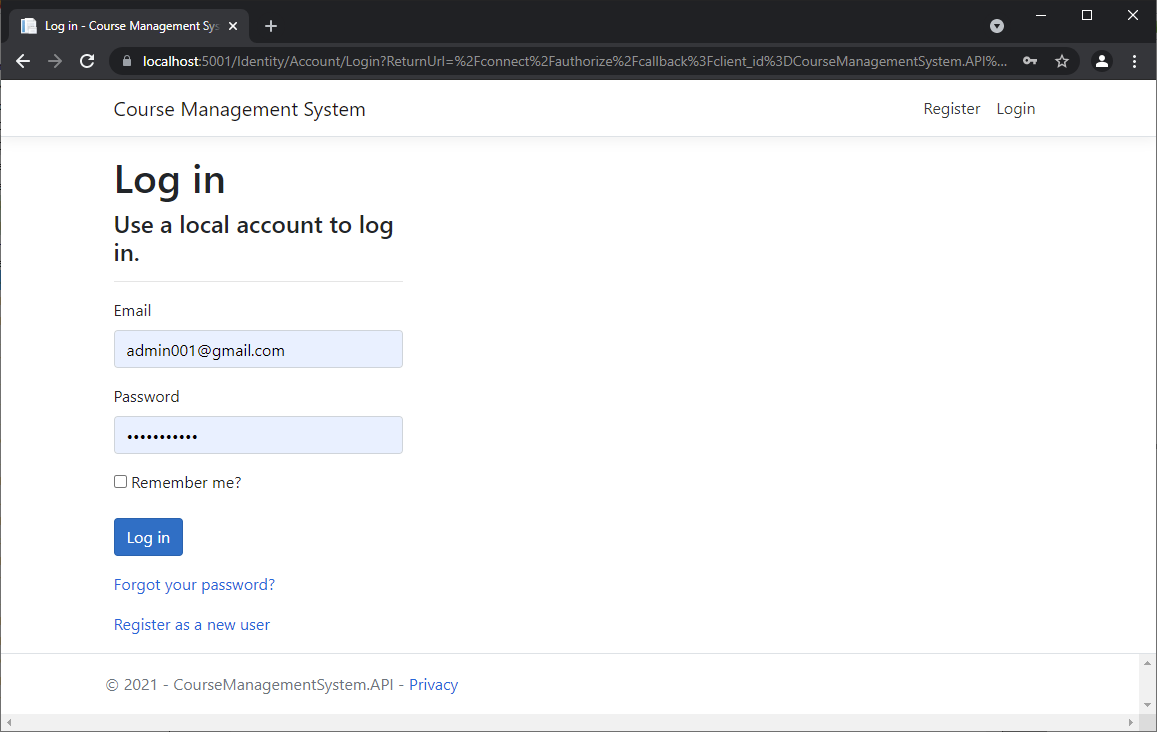
\includegraphics[width=\textwidth]{login-page.PNG}
	\caption{Stránka s přihlášením}
	\label{fig:login}
\end{figure}

\begin{figure}
	\centering
	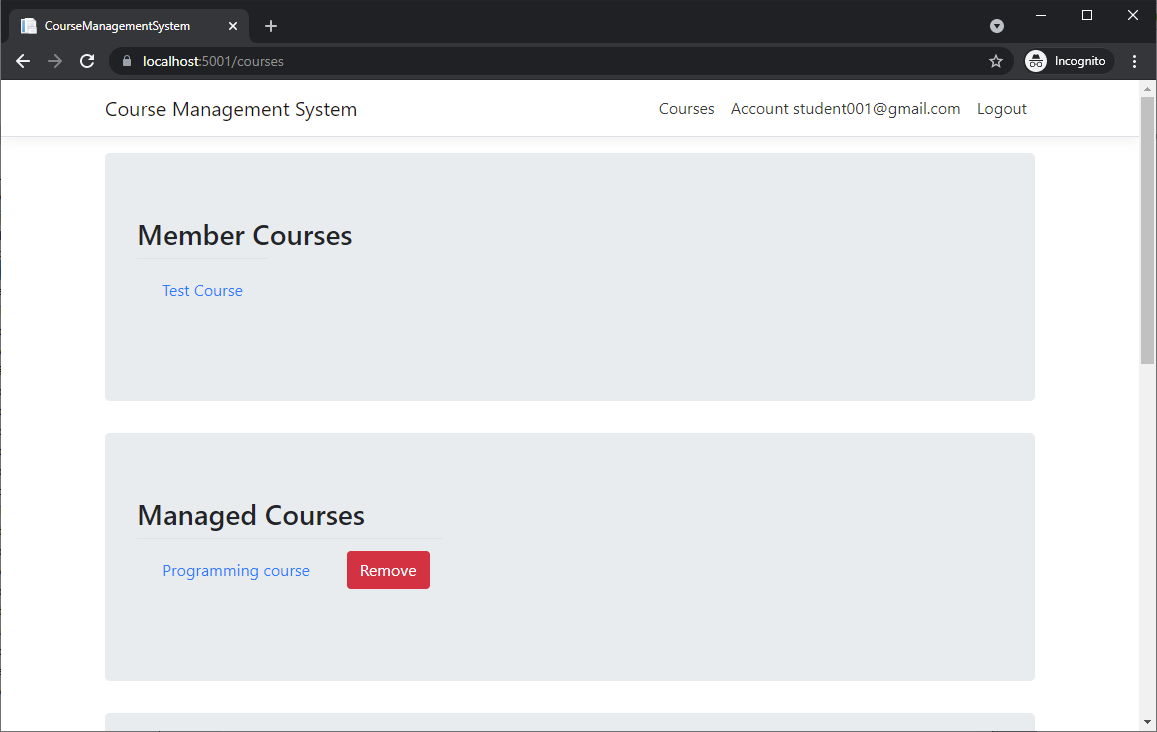
\includegraphics[width=\textwidth]{courses-list.PNG}
	\caption{Stránka se seznamem kurzů}
	\label{fig:courses-list}
\end{figure}

\begin{figure}
	\centering
	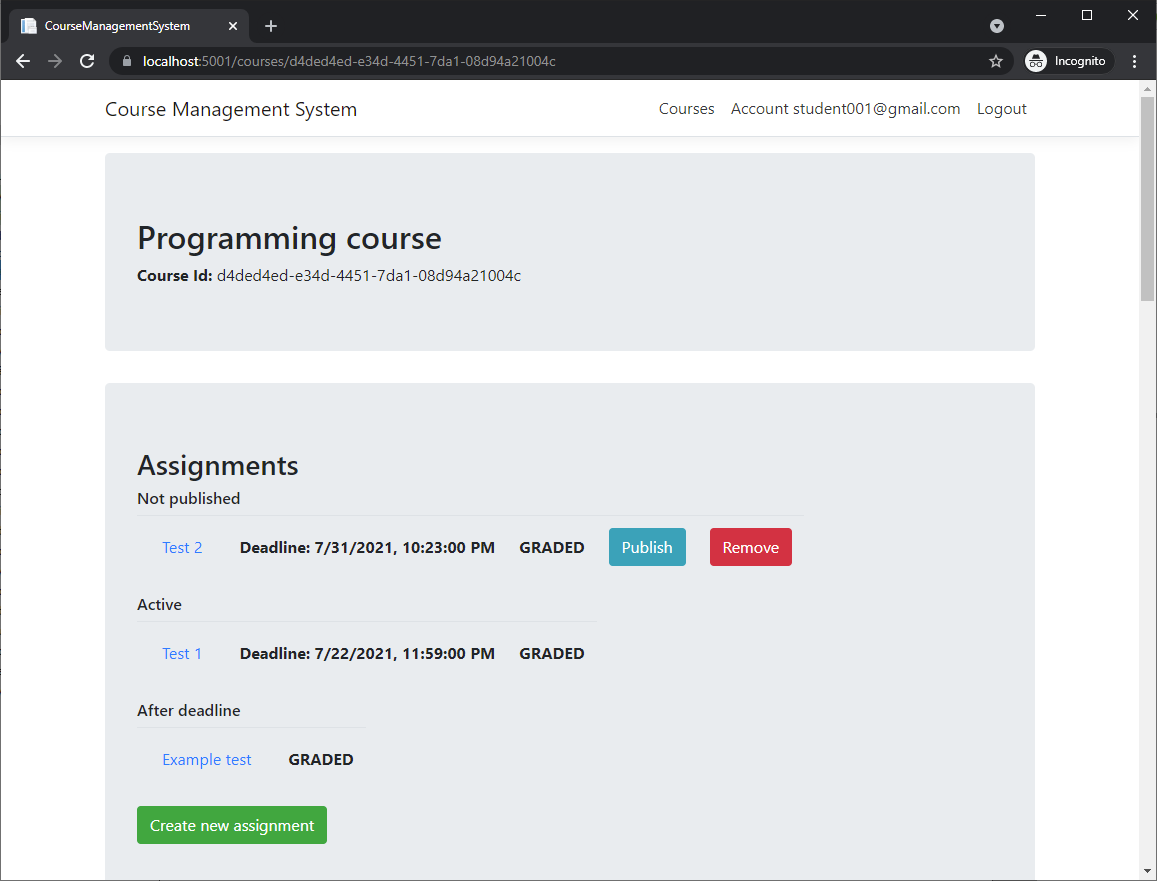
\includegraphics[width=\textwidth]{course-detail.PNG}
	\caption{Stránka s detailem kurzu}
	\label{fig:course-detail}
\end{figure}

\begin{figure}
	\centering
	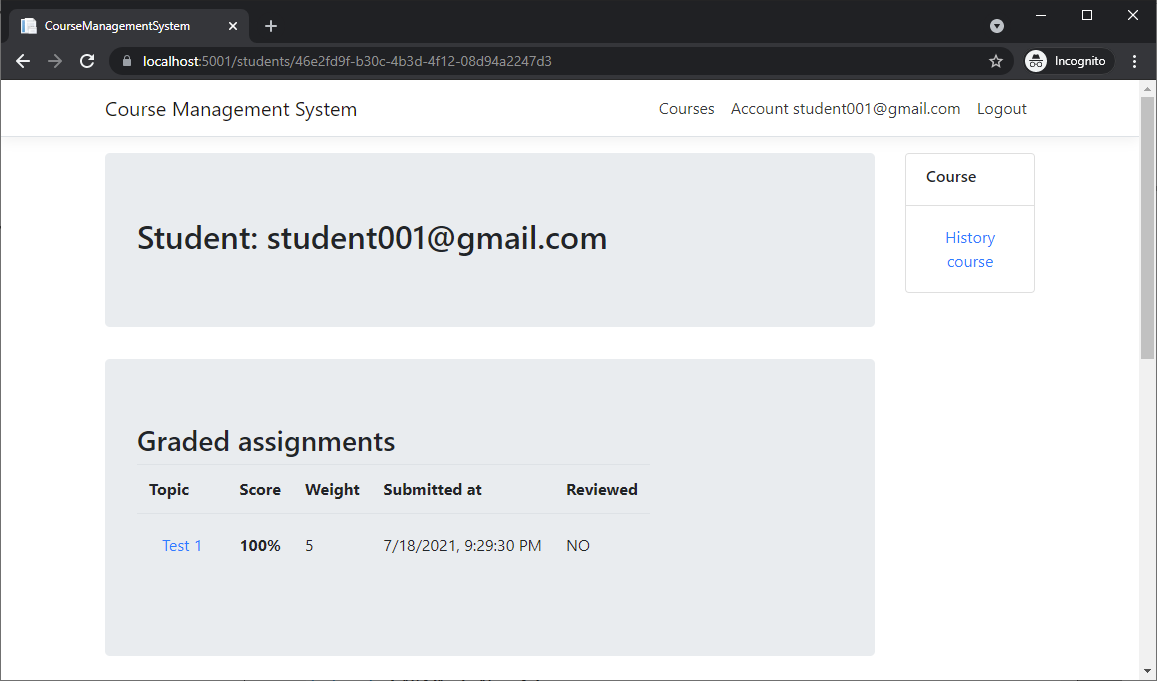
\includegraphics[width=\textwidth]{student-detail.PNG}
	\caption{Stránka s detailem studenta}
	\label{fig:student-detail}
\end{figure}

\begin{figure}
	\centering
	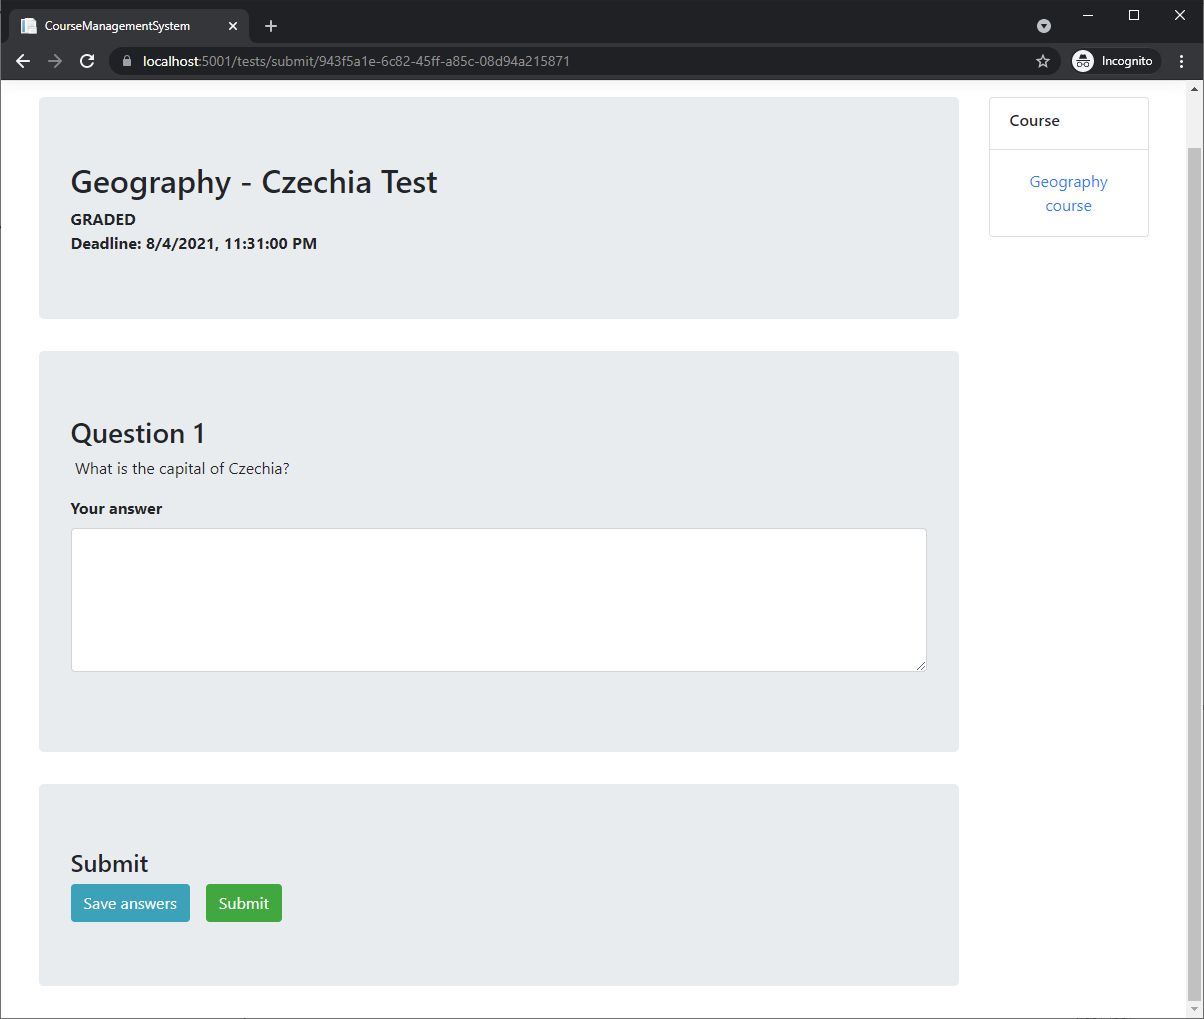
\includegraphics[width=\textwidth]{test-submit.PNG}
	\caption{Stránka s odevzdáním testu}
	\label{fig:test-submit}
\end{figure}

\begin{figure}
	\centering
	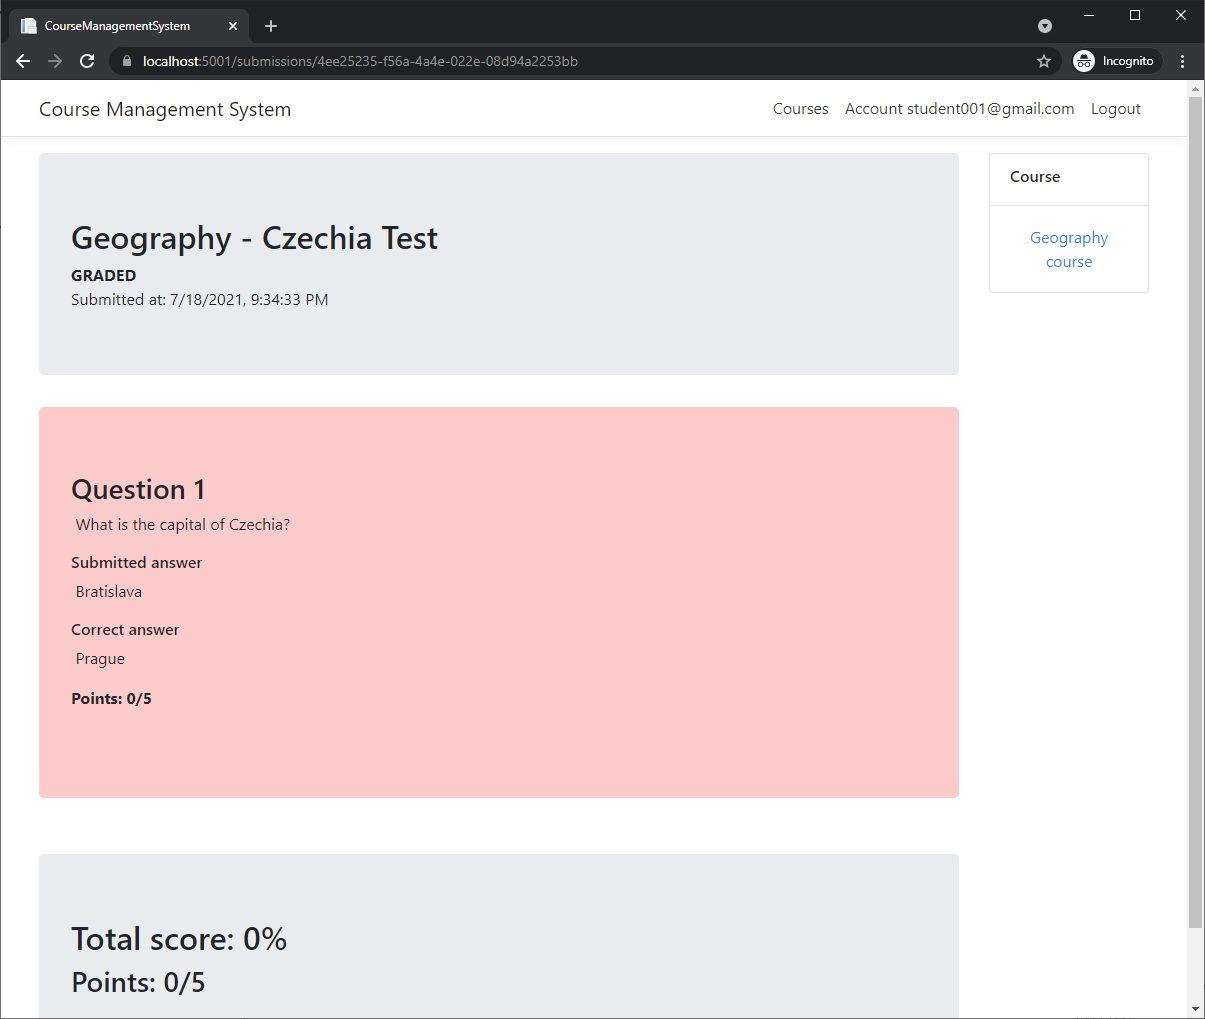
\includegraphics[width=\textwidth]{submission-review.PNG}
	\caption{Zobrazení vyhodnoceného testu}
	\label{fig:submission-review}
\end{figure}

\begin{figure}
	\centering
	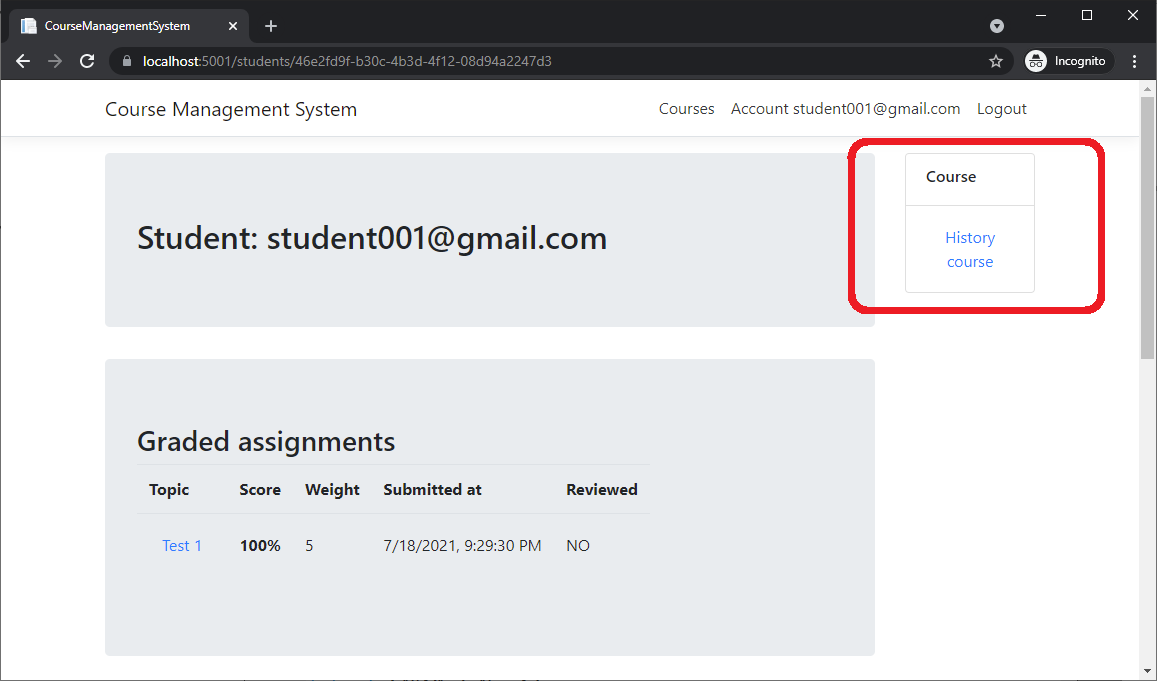
\includegraphics[width=\textwidth]{side-menu.PNG}
	\caption{Postranní menu}
	\label{fig:side-menu}
\end{figure}

\begin{figure}
	\centering
	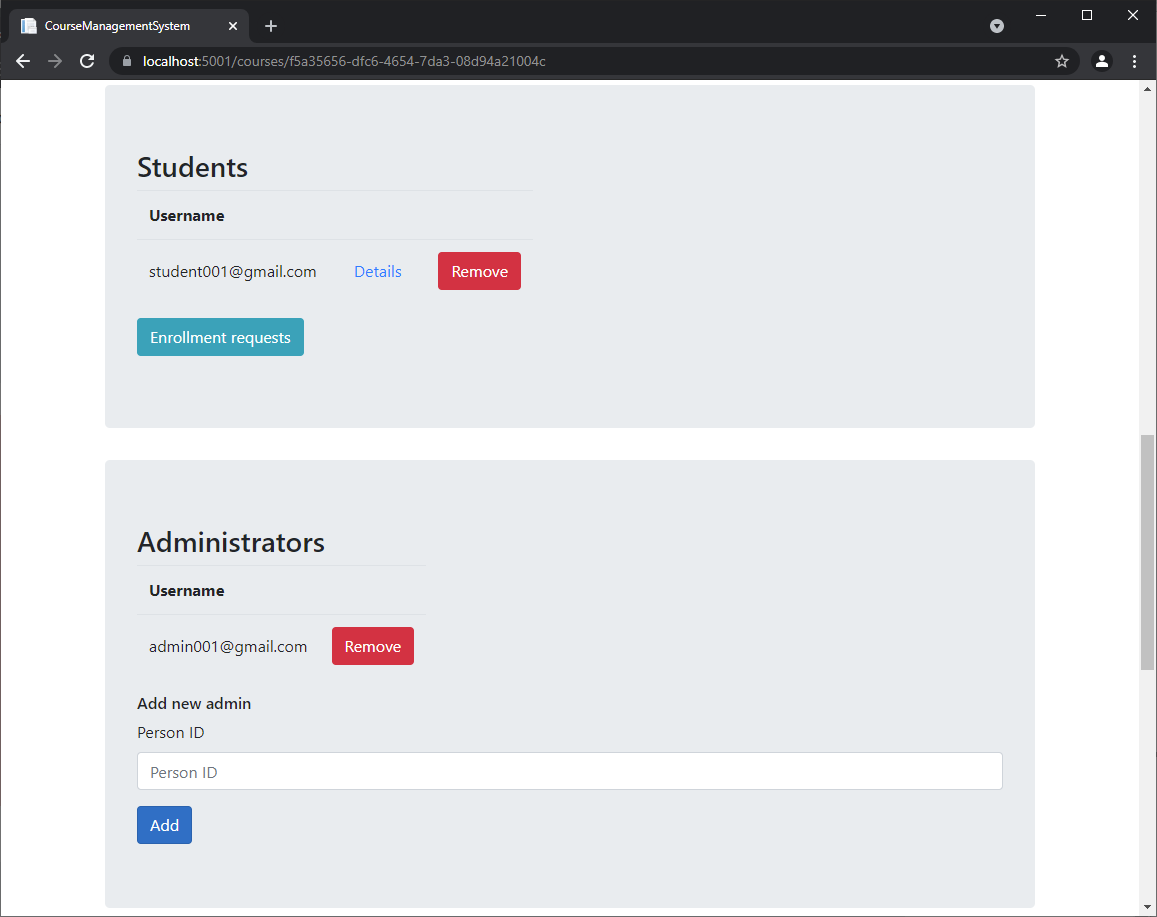
\includegraphics[width=\textwidth]{students-admins-list.PNG}
	\caption{Seznam studentů a administrátorů}
	\label{fig:students-admins-list}
\end{figure}

\begin{figure}
	\centering
	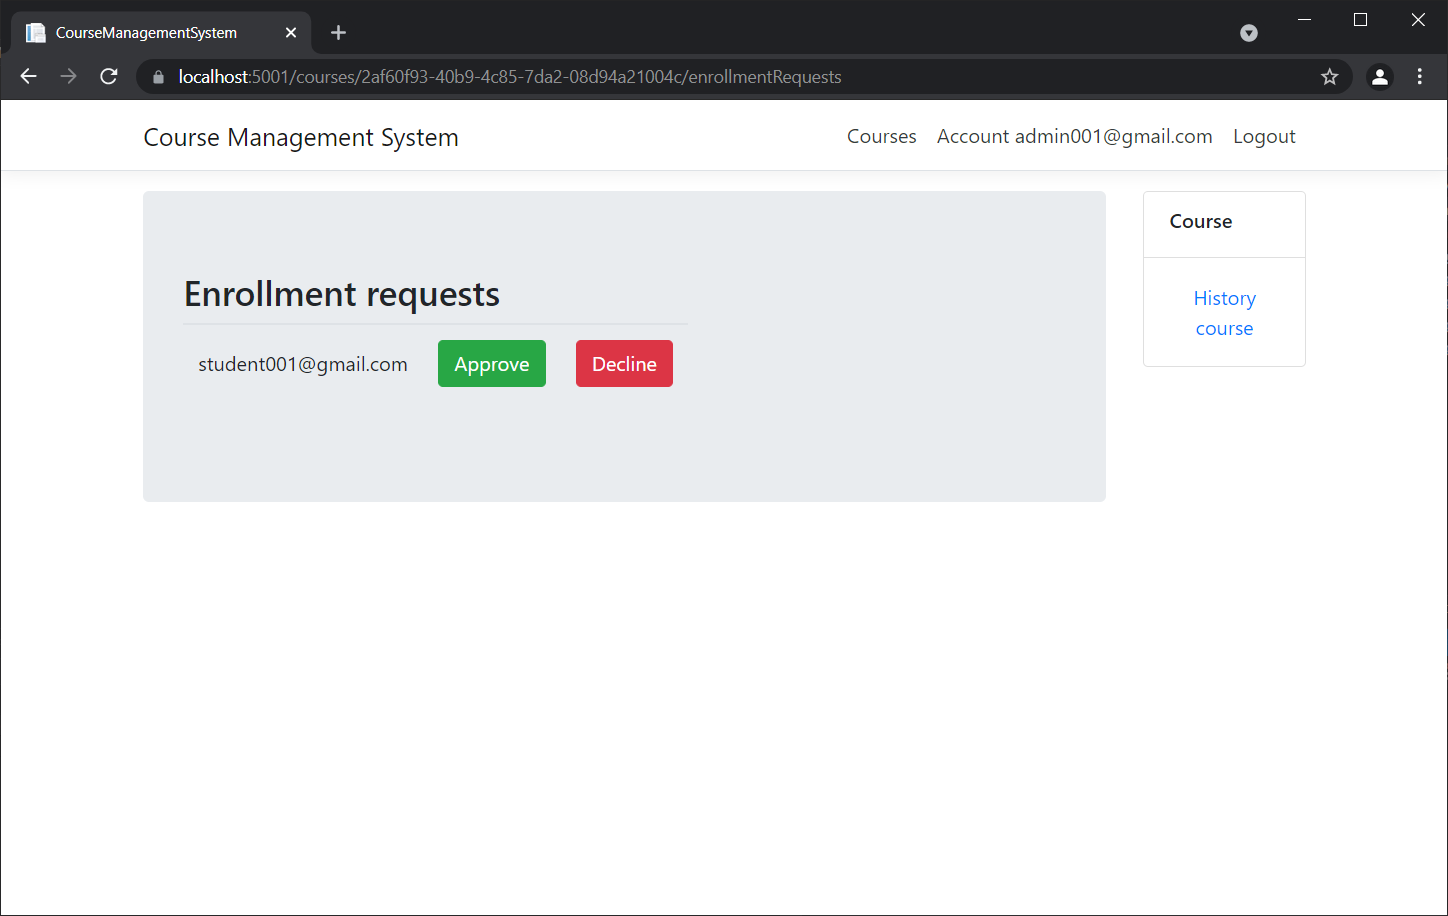
\includegraphics[width=\textwidth]{enrollment-requests.PNG}
	\caption{Seznam žádostí o zápis do daného kurzu}
	\label{fig:enrollment-requests}
\end{figure}

\begin{figure}
	\centering
	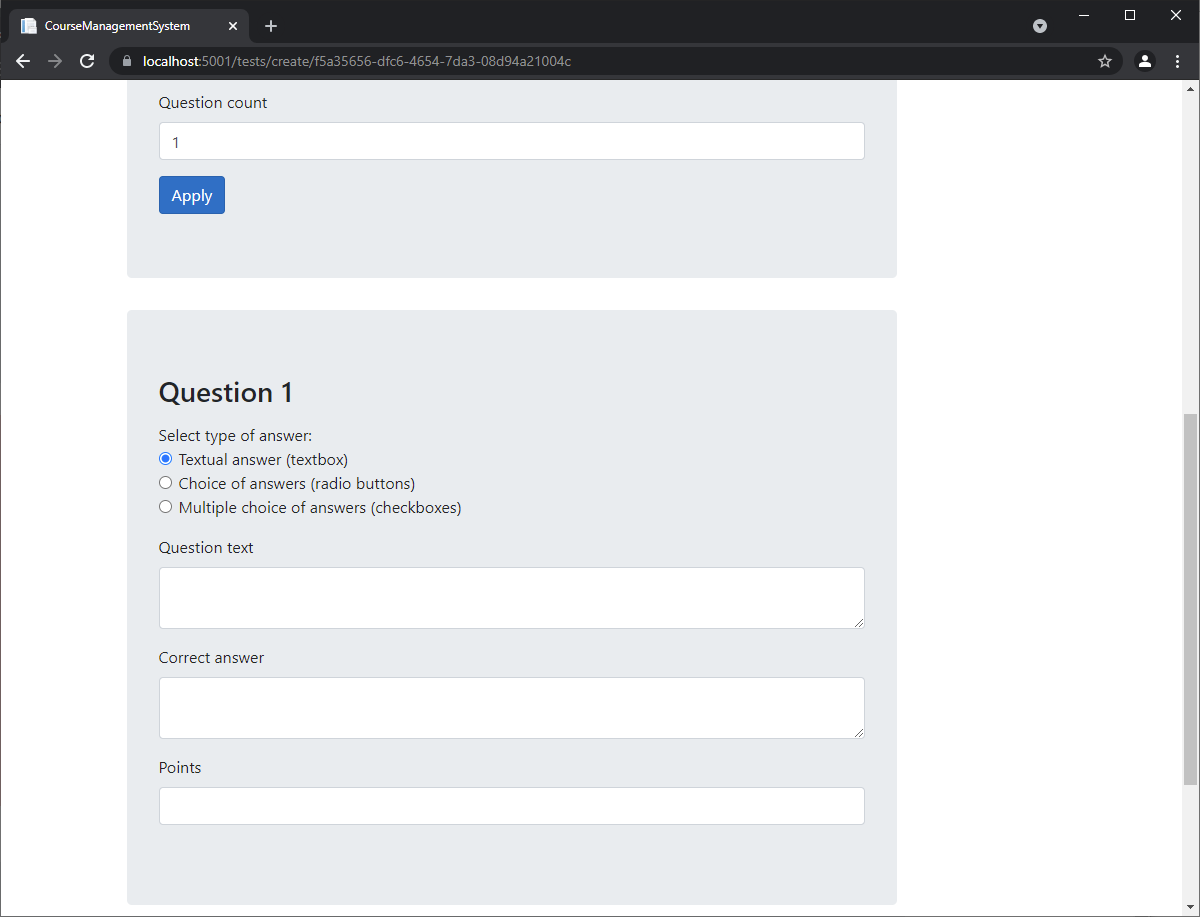
\includegraphics[width=\textwidth]{test-create.PNG}
	\caption{Vytvoření testu}
	\label{fig:test-create}
\end{figure}

\begin{figure}
	\centering
	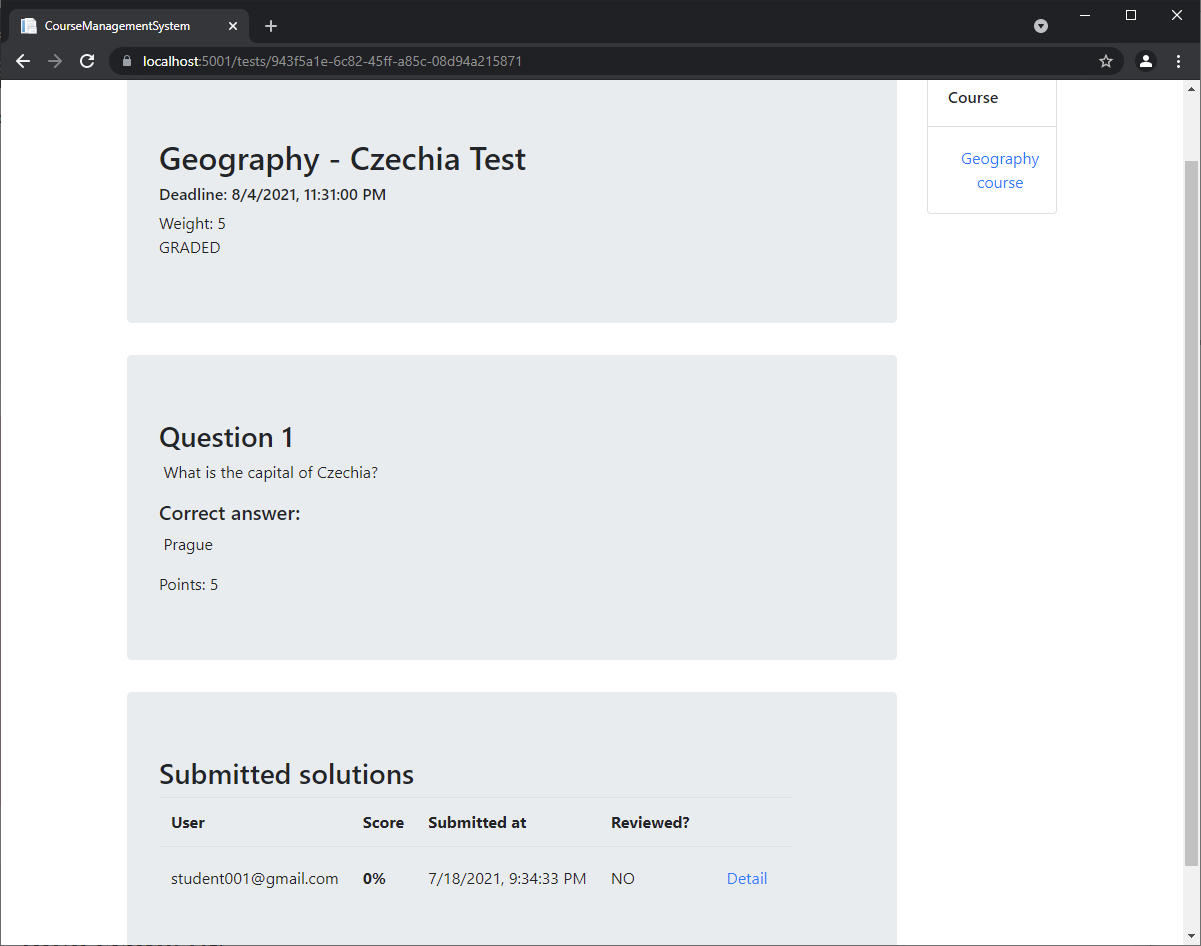
\includegraphics[width=\textwidth]{test-detail.PNG}
	\caption{Stránka s detaily testu}
	\label{fig:test-detail}
\end{figure}

\begin{figure}
	\centering
	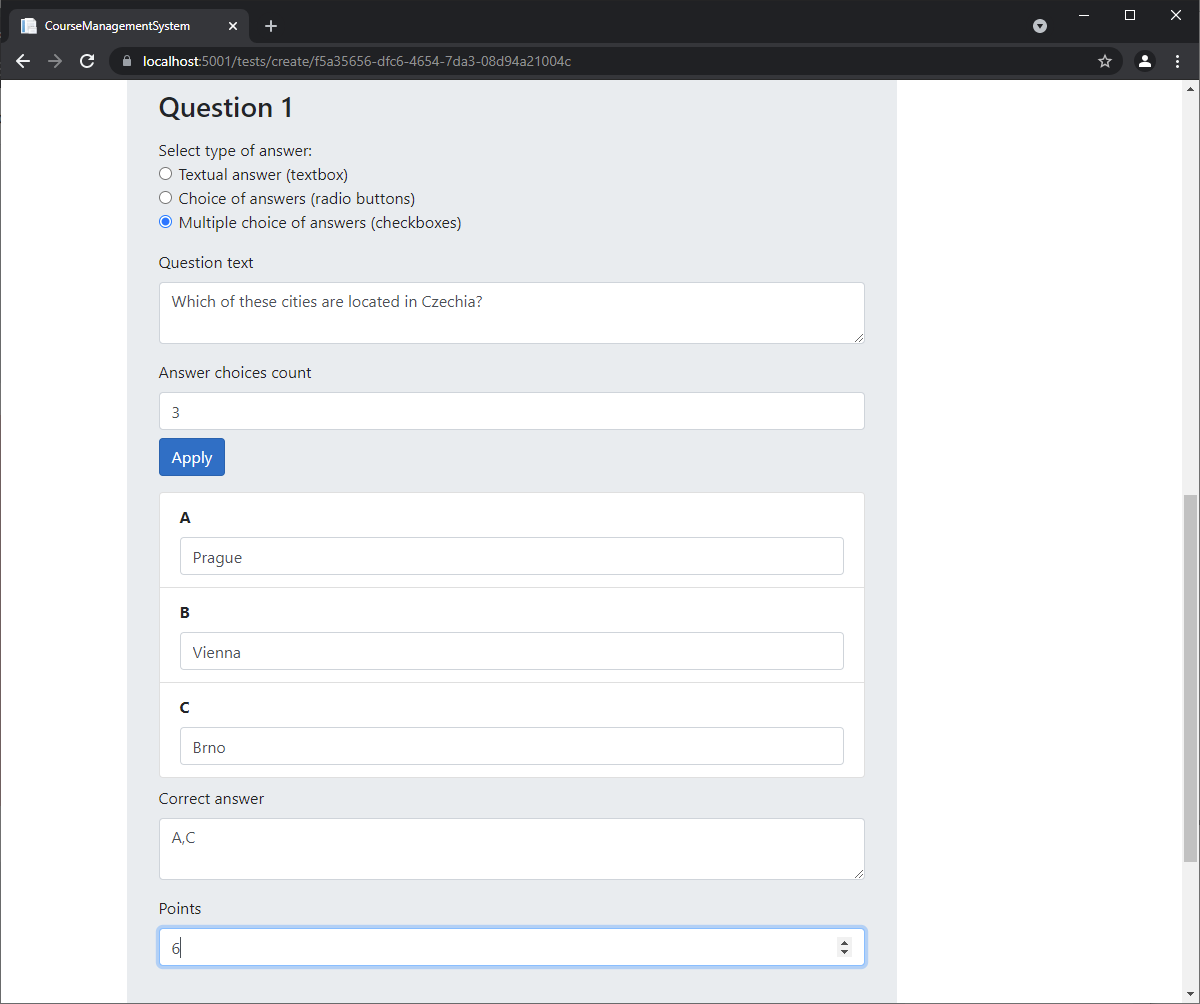
\includegraphics[width=\textwidth]{question-detail.PNG}
	\caption{Vzorová otázka}
	\label{fig:question-detail}
\end{figure}

\begin{figure}
	\centering
	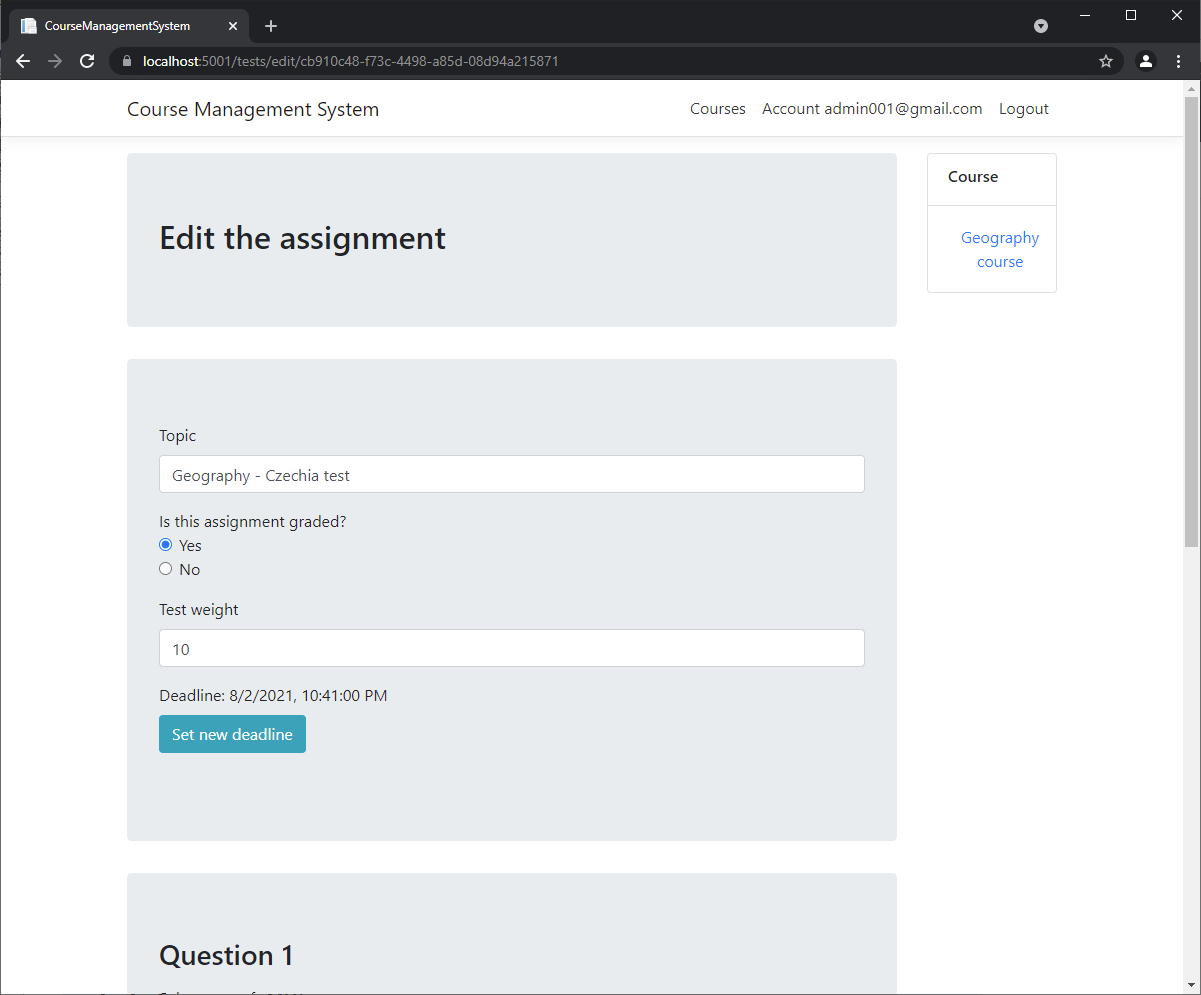
\includegraphics[width=\textwidth]{edit-test1.PNG}
	\caption{Editace testu, část 1}
	\label{fig:test-edit1}
\end{figure}

\begin{figure}
	\centering
	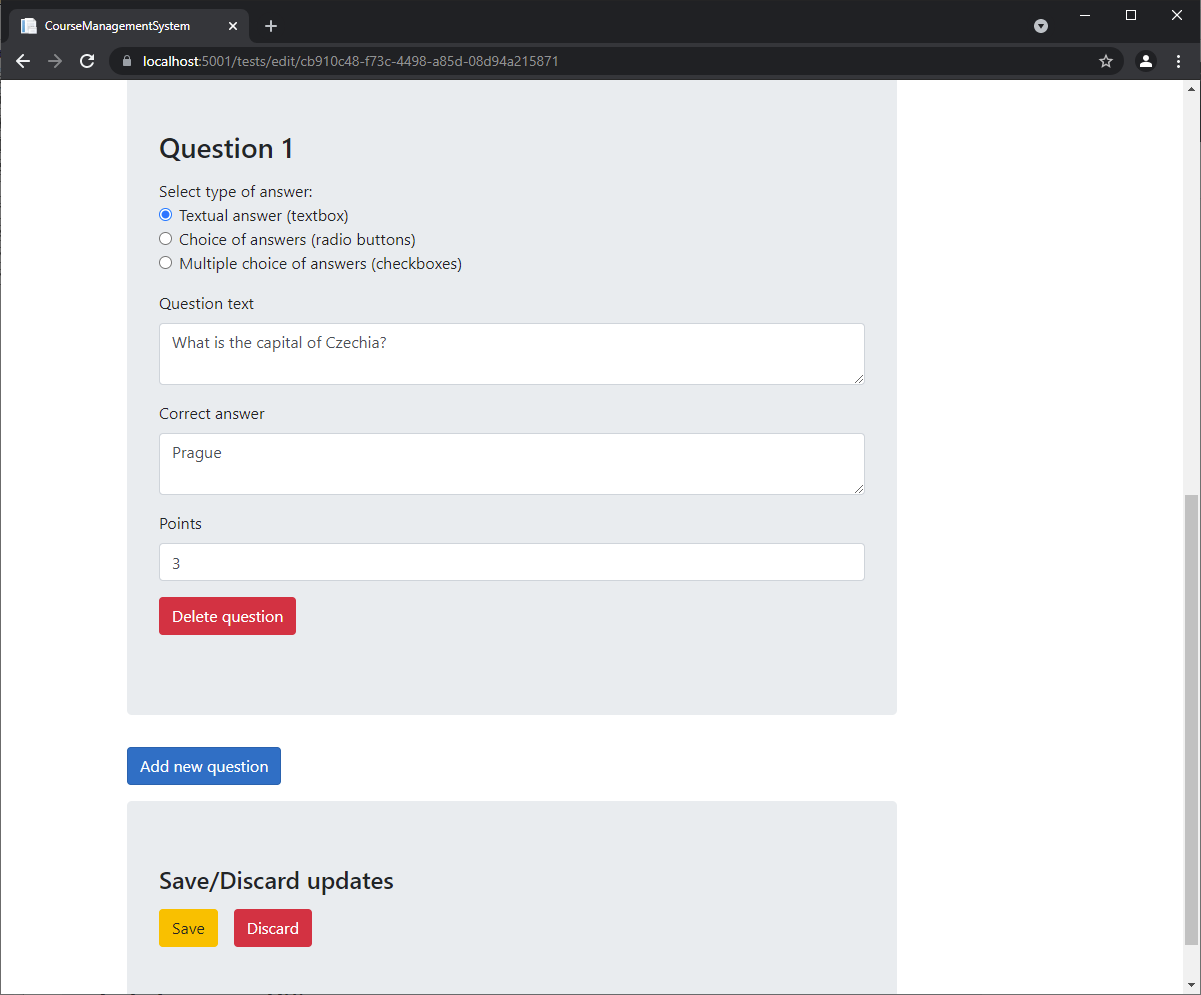
\includegraphics[width=\textwidth]{edit-test2.PNG}
	\caption{Editace testu, část 2}
	\label{fig:test-edit2}
\end{figure}

\begin{figure}
	\centering
	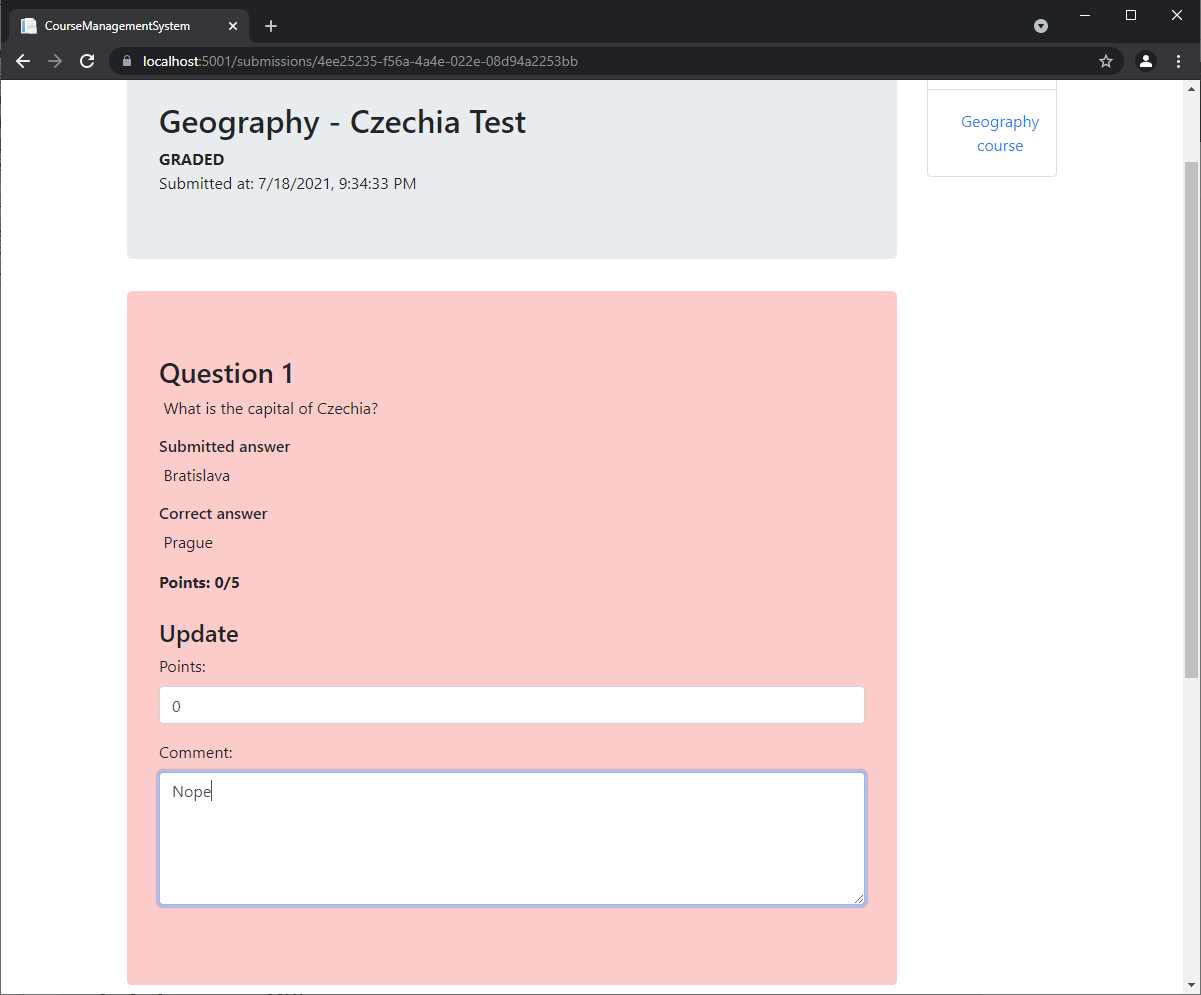
\includegraphics[width=\textwidth]{submission-manual-review.PNG}
	\caption{Manuální oprava odeslaného řešení}
	\label{fig:submission-manual-review}
\end{figure}

\begin{figure}
	\centering
	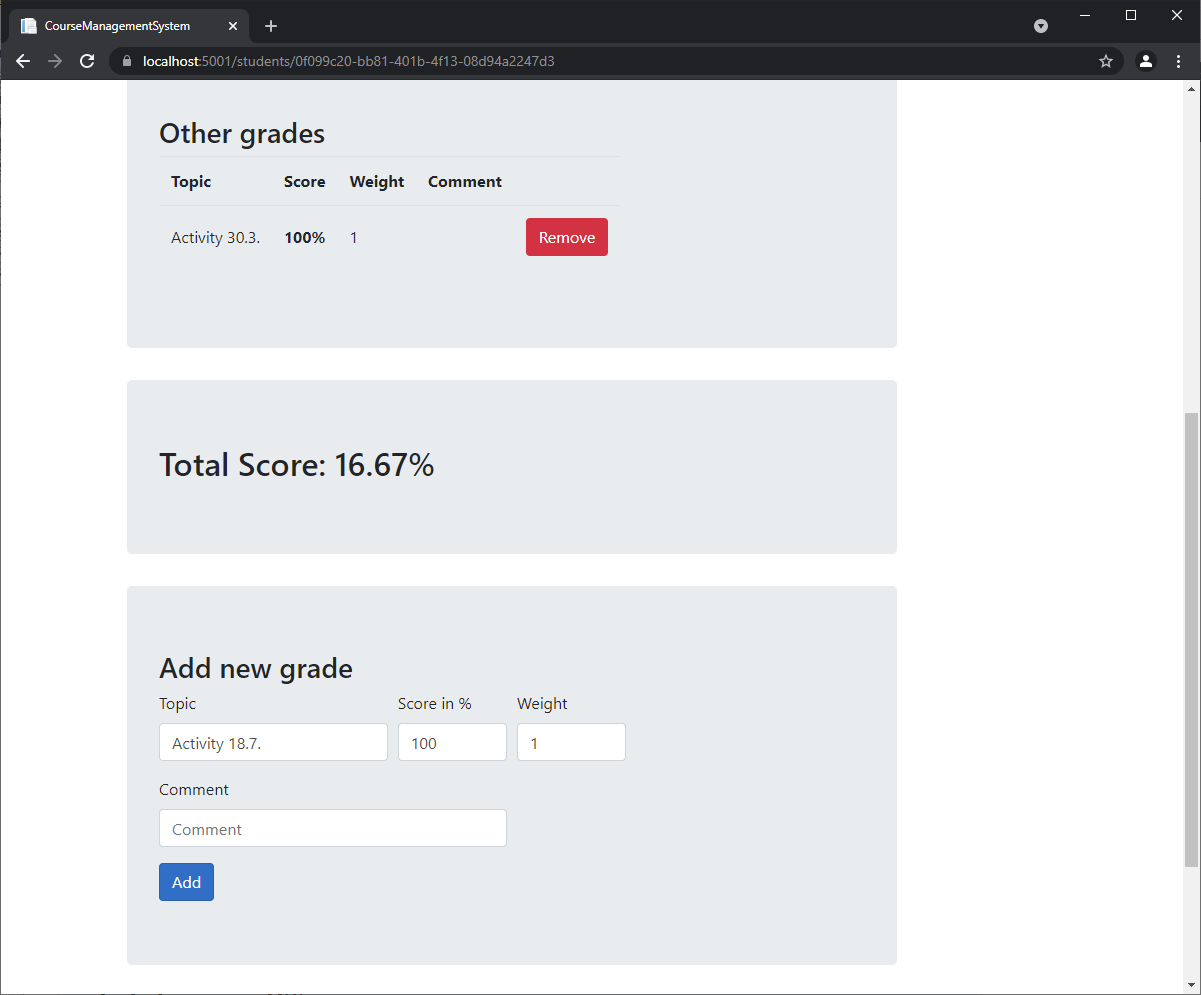
\includegraphics[width=\textwidth]{add-grade.PNG}
	\caption{Formulář pro přidání známky}
	\label{fig:grade-add}
\end{figure}